

\documentclass[table]{article}

\usepackage{graphicx}			% Use this package to include images
\usepackage{amsmath}			% A library of many standard math expressions
\usepackage[margin=0.75in]{geometry}% Sets 1in margins. 
\usepackage{fancyhdr}			% Creates headers and footers
\usepackage{enumerate}          %These two package give custom labels to a list
\usepackage[shortlabels]{enumitem}
\usepackage{tikz}
\usepackage{float} % Add this in your preamble for using [H]

\usepackage{booktabs}
\usepackage{caption}
\usepackage[normalem]{ulem}
\useunder{\uline}{\ul}{}

\usepackage{ragged2e} % Package for justification
\justifying

\graphicspath{{img/}}


\def\mytitle{Homework 2}
\def\righthead{EEF205E}


\usepackage[T1]{fontenc}
\usepackage{lmodern}

%%%%%%%%%%%%%%%%%%%%%%%%%%%%%%%%%%%%%%%%%%%%%%%%%%%%%%%%
\pagestyle{fancy}
\fancyhead[l]{Rüzgar Erik}
\fancyhead[c]{\mytitle}
\fancyhead[r]{\righthead}
\fancyfoot[c]{\thepage}
\renewcommand{\headrulewidth}{0.2pt}
\setlength{\headheight}{15pt}
%%%%%%%%%%%%%%%%%%%%%%%%%%%%%%%%%%%%%%%%%%%%%%%%%%%%%%%%
\usepackage{parskip}
\setlength{\parindent}{0pt} % Disable paragraph indentation
%%%%%%%%%%%%%%%%%%%%%%%%%%%%%%%%%%%%%%%%%%%%%%%%%%%%%%%%


\usepackage{listings}
\usepackage{xcolor}

\lstdefinestyle{verilogstyle}{
    language=Verilog,
    backgroundcolor=\color{white},
    basicstyle=\ttfamily,
    keywordstyle=\color{blue},
    commentstyle=\color{green},
    stringstyle=\color{red},
    numbers=left,
    numberstyle=\tiny\color{gray},
    stepnumber=1,
    numbersep=5pt,
    tabsize=2,
    showspaces=false,
    showstringspaces=false,
}

\lstdefinestyle{vhdlstyle}{
    language=VHDL,
    backgroundcolor=\color{white},
    basicstyle=\ttfamily,
    keywordstyle=\color{blue},
    commentstyle=\color{green},
    stringstyle=\color{red},
    numbers=left,
    numberstyle=\tiny\color{gray},
    stepnumber=1,
    numbersep=5pt,
    tabsize=2,
    showspaces=false,
    showstringspaces=false,
}



\usepackage{karnaugh-map}




\begin{document}


\begin{titlepage}
    \begin{figure}[h] % Places the figure at the right
        \begin{flushright}
        
\includegraphics[width=0.3\textwidth]{logo_laci.png} % Change to your image name
            
        \end{flushright}
        \hfill
    \end{figure}

    \centering
    \vspace*{1in}
    
    \Huge
    \textbf{Introduction to Logic Design} \\
    \textbf{EEF205E} \\

    \vspace{0.5in}

    \Large
    \textbf{\mytitle} \\
    
    \vspace{0.5in}

    \large
    \textbf{Rüzgar Erik} \\
    \textbf{040240783} \\

    \vspace{0.5in}
    
    \Large
    Istanbul Technical University \\
    Faculty of Electrical and Electronics Engineering \\
    
    \vfill


\end{titlepage}



\section*{Part 1}

\begin{enumerate}[label=\textbf{\arabic*.}]
    \item \textbf{Demonstrate the validity of the following identities by means of truth tables:} \\
    
    \begin{enumerate}[label=\textbf{\alph*.}]
        \item \(\left(\left(x  + y +z\right)x \ y\right)' \ = \ x' y' z' + x + y\) \\

        \textbf{Solution:} \\

        \begin{table}[h]
            \centering
            \captionsetup{belowskip=10pt} % Add space below caption
            \caption{Truth Table for the Function \( f(x,y,z) = \left( \left(x  + y +z\right)x \ y\right)'\)} 
            
            \label{tab:my-table}
            \begin{tabular}{|c|c|c|c|c|c|}
                \hline
                \( x \) & \( y \) & \( z \) & \( x + y + z \) & \( (x + y + z) \cdot x \cdot y \) & \( f(x, y, z) = \left( (x + y + z) \cdot x \cdot y \right)' \) \\
                \hline
                0 & 0 & 0 & 0 & 0 & 1 \\
                0 & 0 & 1 & 1 & 0 & 1 \\
                0 & 1 & 0 & 1 & 0 & 1 \\
                0 & 1 & 1 & 1 & 0 & 1 \\
                1 & 0 & 0 & 1 & 0 & 1 \\
                1 & 0 & 1 & 1 & 0 & 1 \\
                1 & 1 & 0 & 1 & 1 & 0 \\
                1 & 1 & 1 & 1 & 1 & 0 \\
                \bottomrule
            \end{tabular}
        \end{table}
        


        Calculating the right side of the equation as \(g(x,y,z) =  x' y' z' + x + y\): \\


        \begin{table}[h]
            \centering
            \caption{Truth Table for the Function \( g(x, y, z) = x' y' z' + x + y \)}
            \begin{tabular}{|c|c|c|c|c|c|c|c|c|}
                \hline
                \( x \) & \( y \) & \( z \) & \( x' \) & \( y' \) & \( z' \) & \( x' y' z' \) & \( x + y \) & \( g(x, y, z) = x' y' z' + x + y \) \\
                \hline
                0 & 0 & 0 & 1 & 1 & 1 & 1 & 0 & 1 \\
                0 & 0 & 1 & 1 & 1 & 0 & 0 & 0 & 0 \\
                0 & 1 & 0 & 1 & 0 & 1 & 0 & 1 & 1 \\
                0 & 1 & 1 & 1 & 0 & 0 & 0 & 1 & 1 \\
                1 & 0 & 0 & 0 & 1 & 1 & 0 & 1 & 1 \\
                1 & 0 & 1 & 0 & 1 & 0 & 0 & 1 & 1 \\
                1 & 1 & 0 & 0 & 0 & 1 & 0 & 1 & 1 \\
                1 & 1 & 1 & 0 & 0 & 0 & 0 & 1 & 1 \\
                \hline
            \end{tabular}
        \end{table}

        As seen from the truth tables the given equation is not valid. The non-equal rows are colored red in the Table \ref{tab:combined-table}\\

        \begin{table}[h]
            \centering
            \caption{Combined Truth Table for \( f(x, y, z) = \left( (x + y + z) \cdot x \cdot y \right)' \) and \( g(x, y, z) = x' y' z' + x + y \)}
            \label{tab:combined-table}
            \begin{tabular}{|c|c|c|c|c|}
                \hline
                \( x \) & \( y \) & \( z \) & \( f(x, y, z) = \left( (x + y + z) \cdot x \cdot y \right)' \) & \( g(x, y, z) = x' y' z' + x + y \) \\
                \hline
                0 & 0 & 0 & 1 & 1 \\
               \rowcolor{red} 0 & 0 & 1 & 1 & 0 \\
                0 & 1 & 0 & 1 & 1 \\
                0 & 1 & 1 & 1 & 1 \\
                1 & 0 & 0 & 1 & 1 \\
                1 & 0 & 1 & 1 & 1 \\
                \rowcolor{red} 1 & 1 & 0 & 0 & 1 \\
                \rowcolor{red} 1 & 1 & 1 & 0 & 1 \\
                \hline
            \end{tabular}
        \end{table}
        
        \newpage

        \item \(x(x' + y + z) = xy + xz\) \\
        
        \textbf{Solution:} \\


        \begin{table}[h]
            \centering
            \captionsetup{belowskip=10pt} % Add space below caption
            \caption{Combined Truth Table for \( f(x, y, z) \), \( g(x, y, z) \), and \( h(x, y, z) = x(x' + y + z) \)}
            \label{tab:combined-functions}
            \begin{tabular}{|c|c|c|c|c|c|c|c|c|}
                


                \hline

                \( x \) & \( y \) & \( z \) & \( x' \) & \( x' + y + z \) & \( f(x, y, z) = x(x' + y + z) \) & \( xy \) & \( xz \) & \( g(x, y, z) = xy + xz \) \\
                \hline


                0 & 0 & 0 & 1 & 1 & 0 & 0 & 0 & 0 \\
                0 & 0 & 1 & 1 & 1 & 0 & 0 & 0 & 0 \\
                0 & 1 & 0 & 1 & 1 & 0 & 0 & 0 & 0 \\
                0 & 1 & 1 & 1 & 1 & 0 & 0 & 0 & 0 \\
                1 & 0 & 0 & 0 & 0 & 0 & 0 & 0 & 0 \\
                1 & 0 & 1 & 0 & 1 & 1 & 0 & 1 & 1 \\
                1 & 1 & 0 & 0 & 1 & 1 & 1 & 0 & 1 \\
                1 & 1 & 1 & 0 & 1 & 1 & 1 & 1 & 1\\
        
                \hline
            \end{tabular}
        \end{table}

        By comparing the truth tables of the functions \( f(x, y, z) = x(x' + y + z) \) and \( g(x, y, z) = xy + xz \) in Table \ref{tab:combined-functions}, it can be seen that the given equation is valid.

    \end{enumerate}


    \item \textbf{Simplify the following Boolean expressions to a minimum number of literals:}
    

    \begin{enumerate}[label=\textbf{\alph*.}]
        \item \(\mathbf{ABC + A'B + ABC'}\) \\
        
        \textbf{Solution:} \\
        
        \begin{align*}
            ABC + A'B + ABC' & = AB(C + C') + A'B \\
            & = AB + A'B \\
            & = B(A + A') \\
            & = B
        \end{align*}

        \item \(\mathbf{\left(x+y\right)' \ \left(x' + y'\right)}\) \\
        
        \textbf{Solution:} \\

        \begin{align*}
            \left(x+y\right)' \ \left(x' + y'\right) &= x'y' \cdot \left(x'+y'\right) \\
            &= (x'y'x') + (x'y'y') \\
            &= (x'y') + (x'y') \\
            &= x'y'
        \end{align*}


        \item \(\mathbf{xy + x \left(wz + wz'\right)}\) \\
        
        \textbf{Solution:} \\

        \begin{align*}
            xy + x \left(wz + wz'\right) &= xy + xw(z + z') \\
            &= xy + xw \\
        \end{align*}

        \item \(\mathbf{\left(a' + c'\right)\left(a + b' + c'\right)}\) \\
        
        \textbf{Solution:} \\

        \begin{align*}
            (a' + c')(a + b' + c') &= a(a' + c') + b'(a' + c') + c'(a' + c') \\
            &= (aa' + ac') + (a'b' + b'c') + (c'a' + c'c')\\
            &= (0 + ac') + (a'b' + b'c') + (a'c' + c') \\
            &= ac' + a'b' + b'c' + a'c' + c'
            &= c'(a + b' + a' + 1) + a'b' \\
            &= c' + a'b'
        \end{align*}



    \end{enumerate}

    \item \textbf{Boolean functions for the outputs \(c_2(a_1,a_0,b_1,b_0)\), \(c_1(a_1,a_0,b_1,b_0)\) and \(c_0(a_1,a_0,b_1,b_0)\) shown by the below truth table will be implemented in Part 2. } 
    
    \begin{table}[h!]
        \centering
       \caption{Truth Table for the Outputs \(c_2\), \(c_1\), and \(c_0\)}
       \label{tab:truth-given}
       \begin{tabular}{|r|c|c|c|c||c|c|c|}
       \hline
       \textbf{Index} & $a_1$ & $a_0$ & $b_1$ & $b_0$ & $c_2$ & $c_1$ & $c_0$ \\
       \hline
       \textbf{0} & 0 & 0 & 0 & 0 & 0 & 0 & 0 \\
       \textbf{1} & 0 & 0 & 0 & 1 & 0 & 0 & 1 \\
       \textbf{2} & 0 & 0 & 1 & 0 & 0 & 1 & 0 \\
       \textbf{3} & 0 & 0 & 1 & 1 & 0 & 1 & 1 \\
       \textbf{4} & 0 & 1 & 0 & 0 & 0 & 0 & 1 \\
       \textbf{5} & 0 & 1 & 0 & 1 & 0 & 1 & 0 \\
       \textbf{6} & 0 & 1 & 1 & 0 & 0 & 1 & 1 \\
       \textbf{7} & 0 & 1 & 1 & 1 & 1 & 0 & 0 \\
       \textbf{8} & 1 & 0 & 0 & 0 & 0 & 1 & 0 \\
       \textbf{9} & 1 & 0 & 0 & 1 & 0 & 1 & 1 \\
       \textbf{10} & 1 & 0 & 1 & 0 & 1 & 0 & 0 \\
       \textbf{11} & 1 & 0 & 1 & 1 & 1 & 0 & 1 \\
       \textbf{12} & 1 & 1 & 0 & 0 & 0 & 1 & 1 \\
       \textbf{13} & 1 & 1 & 0 & 1 & 1 & 0 & 0 \\
       \textbf{14} & 1 & 1 & 1 & 0 & 1 & 0 & 1 \\
       \textbf{15} & 1 & 1 & 1 & 1 & 1 & 1 & 0 \\
       \hline
       \end{tabular}
       \end{table}



    \begin{enumerate}[label=\textbf{\alph*.}]
        \item Find sum of products expressions for \(c_2\), \(c_1\), and \(c_0\). \\
        
        \textbf{Solution:} \\

        \begin{enumerate}[label=\textbf{\roman* .}]
            \item SOP for \(c_2\) \\
        
            Firstly the minterms for \(c_2\) are found by looking at the rows where \(c_2 = 1\). The minterms are \(7\), \(10\), \(11\), \(13\), \(14\), \(15\) The sum of products expression for \(c_2\) is: \\
            
            \begin{align*}
                c_2 &= \Sigma(7, 10, 11, 13, 14, 15) = a_1'a_0b_1b_0 + a_1a_0'b_1b_0' + a_1a_0'b_1b_0 + a_1a_0b_1'b_0 + a_1a_0b_1b_0' + a_1a_0b_1b_0
            \end{align*}

            \item SOP for \(c_1\) \\
            
            The minterms for \(c_1\) are \(2\), \(3\), \(5\), \(6\), \(8\), \(9\), \(12\), \(15\). The sum of products expression for \(c_1\) is: \\
            
            \begin{align*}
                c_1 &= \Sigma(2, 3, 5, 6, 8, 9, 12, 15) \\
                    &= a_1'a_0'b_1b_0' + a_1'a_0'b_1b_0 + a_1'a_0b_1'b_0 + a_1'a_0b_1b_0' \\
                    &\quad + a_1a_0'b_1'b_0' + a_1a_0'b_1'b_0 + a_1a_0b_1'b_0' + a_1a_0b_1b_0 
            \end{align*}
            

            \item SOP for \(c_0\) \\
            
            The minterms for \(c_0\) are \(1\), \(3\), \(4\), \(6\), \(9\), \(11\), \(12\), \(14\). The sum of products expression for \(c_0\) is: \\
            
            
            \begin{align*}
                c_0 &= \Sigma(1, 3, 4, 6, 9, 11, 12, 14) \\
                    &= a_1'a_0'b_1'b_0 + a_1'a_0'b_1b_0 + a_1'a_0b_1'b_0' + a_1'a_0b_1b_0' \\
                    &\quad + a_1a_0'b_1'b_0 + a_1a_0'b_1b_0 + a_1a_0b_1'b_0' + a_1a_0b_1b_0'
            \end{align*}

        \end{enumerate} %part a solutions enumeration

        \item \textbf{Simplify the sum of products expressions for \(c_2\), \(c_1\), and \(c_0\).} \\
        
        \textbf{Solution:} \\

        \begin{enumerate}[label=\textbf{\roman* .}]
            \item Solving for \(c_2\) \\
            
            Karnaugh map method was chosen to simplify the sum of products expression for all of the questions. The Karnaugh map for \(c_2\) is shown in Figure \ref{fig:kmap-c2}.

            \begin{figure}[H]
                \centering

            \begin{karnaugh-map}(label=corner)[4][4][1][\(b_0\)][\(b_1\)][\(a_0\)][\(a_1\)]
                \minterms{7, 10, 11, 13, 14, 15}
                \maxterms{0, 1, 2, 3, 4, 5, 6, 8, 9, 12}
                \implicant{7}{15}
                \implicant{15}{10}
                \implicant{13}{15}
            \end{karnaugh-map}

            \caption{Karnaugh Map for \(c_2\)}
            \label{fig:kmap-c2}

            \end{figure}

            The simplified sum of products expression for \(c_2\) is: \(c_2 = a_0b_1b_0 + a_1b_1 + a_1a_0b_0\)
            \newpage

            \item Solving for \(c_1\) \\
            
            The Karnaugh map for \(c_1\) is shown in Figure \ref{fig:kmap-c1}.

            \begin{figure}[H]
                \centering

            \begin{karnaugh-map}(label=corner)[4][4][1][\(b_0\)][\(b_1\)][\(a_0\)][\(a_1\)]
                
                \minterms{2, 3, 5, 6, 8, 9, 12, 15}
                \maxterms{0, 1, 4, 7, 10, 11, 13, 14}
                \implicant{3}{2}
                \implicant{2}{6}
                \implicant{5}{5}
                \implicant{12}{8}
                \implicant{8}{9}
                \implicant{15}{15}
            \end{karnaugh-map}

            \caption{Karnaugh Map for \(c_1\)}
            \label{fig:kmap-c1}

            \end{figure}

            The simplified sum of products expression for \(c_1\) is: \(c_1 = a_1'a_0'b_1 + a_1'a_0b_1'b_0 + a_1'b_1b_0' + a_1a_0'b_1' + a_1b_1'b_0' + a_1a_0b_1b_0  \) 

            \item Solving for \(c_0\) \\
            
            The Karnaugh map for \(c_0\) is shown in Figure \ref{fig:kmap-c0}.

            \begin{figure}[H]
                \centering

            \begin{karnaugh-map}(label=corner)[4][4][1][\(b_0\)][\(b_1\)][\(a_0\)][\(a_1\)]
                \minterms{1, 3, 4, 6, 9, 11, 12, 14}
                \maxterms{0, 2, 5, 7, 8, 10, 13, 15}
                \implicantedge{4}{12}{6}{14}
                \implicantedge{1}{3}{9}{11}

            \end{karnaugh-map}

            \caption{Karnaugh Map for \(c_0\)}
            \label{fig:kmap-c0}

            \end{figure}

            The simplified sum of products expression for \(c_0\) is: \(c_0 =  a_0'b_0 + a_0b_0'\)

        \end{enumerate} %SOP simplification enumeration

    \end{enumerate}



\end{enumerate} %parts enumeration

\newpage


\section*{Part 2}

\subsection*{Boolean Function Case Statement }


Using the truth table a behavioral model for the circuit is implemented in VHDL. The code is shown below:


\begin{center} % Center the entire code block
    \lstset{
  caption= Boolean\_Function\_Case\_Statement.vhd, 
  basicstyle=\footnotesize, frame=tb,
  xleftmargin=.2\textwidth, xrightmargin=.2\textwidth
}
    \lstinputlisting[style=vhdlstyle]{code/Boolean_Function_Case_Statement.vhd}

\end{center}

\subsubsection*{Testbench for the Boolean Function Case Statement}

The testbench for the behavioral model is implemented in VHDL. The code is shown below:

\begin{center} % Center the entire code block
    \lstset{
  caption= Boolean\_Function\_Case\_Statement\_tb.vhd, 
  basicstyle=\footnotesize, frame=tb,
  xleftmargin=.2\textwidth, xrightmargin=.2\textwidth
}
    \lstinputlisting[style=vhdlstyle]{code/Boolean_Function_Case_Statement_tb.vhd}

\end{center}

\newpage
\subsubsection*{RTL Schematic of the Boolean Function Case Statement}

The RTL schematic of the behavioral model is shown in Figure \ref{fig:rtl-schematic}.
\begin{figure}[H]
    \centering
    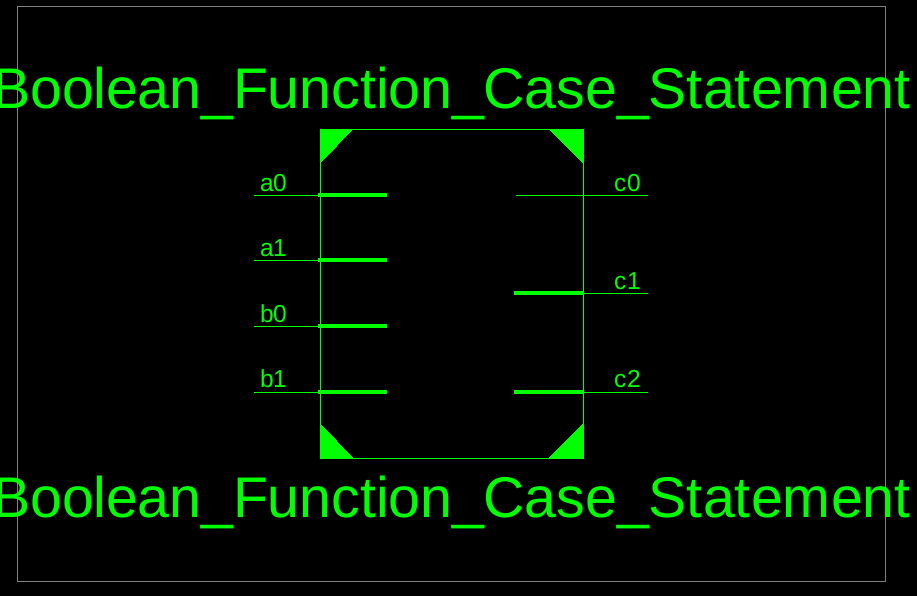
\includegraphics[width=0.3\textwidth]{img/rtltop.png}
    \caption{RTL Schematic of the Boolean Function Case Statement}
    \label{fig:rtl-schematic}
\end{figure}

Going one more layer deep, the schematic of the individual components of the behavioral model is shown in Figure \ref{fig:rtl-schematic-components}.

\begin{figure}[H]
    \centering
    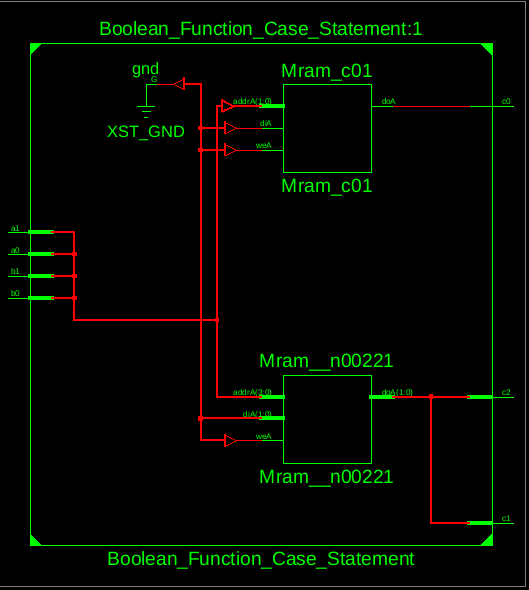
\includegraphics[width=0.4\textwidth]{img/RTLLAYER.png}
    \caption{RTL Schematic of the Components of the Boolean Function Case Statement}
    \label{fig:rtl-schematic-components}

\end{figure}


\subsubsection*{Simulation Results}

The simulation results of the testbench for the behavioral model is shown in Figure \ref{fig:simulation-results}.

\begin{figure}[H]
    \centering
    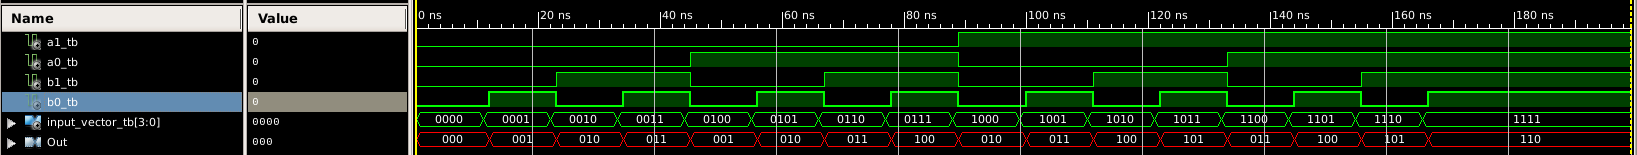
\includegraphics[width=0.75\textwidth]{img/anakod3.png}
    \caption{Simulation Results of the Testbench for the Boolean Function Case Statement}
    \label{fig:simulation-results}
\end{figure}

It can be seen that from inputs at the bottom of the waveform, the outputs \(c_2\), \(c_1\), and \(c_0\) are as expected from the truth table in Table \ref{tab:truth-given}.

\newpage

\subsection*{Dataflow Model}

The dataflow model for the circuit is implemented in VHDL. The code is shown below:

\begin{center} % Center the entire code block
    \lstset{
  caption= Boolean\_Function\_Data\_Flow.vhd, 
  basicstyle=\footnotesize, frame=tb,
  xleftmargin=.2\textwidth, xrightmargin=.2\textwidth
}
    \lstinputlisting[style=vhdlstyle]{code/Boolean_Function_Data_Flow.vhd}

\end{center}

\subsubsection*{Testbench for the Boolean Function Data Flow}

The testbench for the dataflow model is implemented in VHDL. The code is shown below:

\begin{center} % Center the entire code block
    \lstset{
  caption= Boolean\_Function\_Data\_Flow\_tb.vhd, 
  basicstyle=\footnotesize, frame=tb,
  xleftmargin=.2\textwidth, xrightmargin=.2\textwidth
}
    \lstinputlisting[style=vhdlstyle]{code/Boolean_Function_Data_Flow_tb.vhd}


\end{center}

\subsubsection{RTL Schematic of the Boolean Function Data Flow}

The RTL schematic of the dataflow model is shown in Figure \ref{fig:rtl-schematic-dataflow}.

\begin{figure}[H]
    \centering
    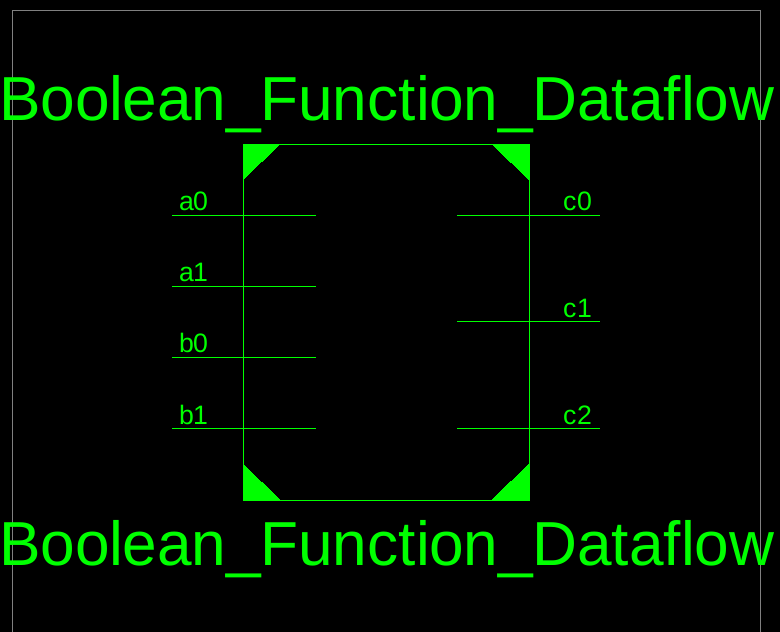
\includegraphics[width=0.45\textwidth]{img/rtl_df_1.png}
    \caption{RTL Schematic of the Boolean Function Data Flow}
    \label{fig:rtl-schematic-dataflow}
\end{figure}

The schematic of the individual components of the dataflow model is shown in Figure \ref{fig:rtl-schematic-components-dataflow}.

\begin{figure}[H]
    \centering
    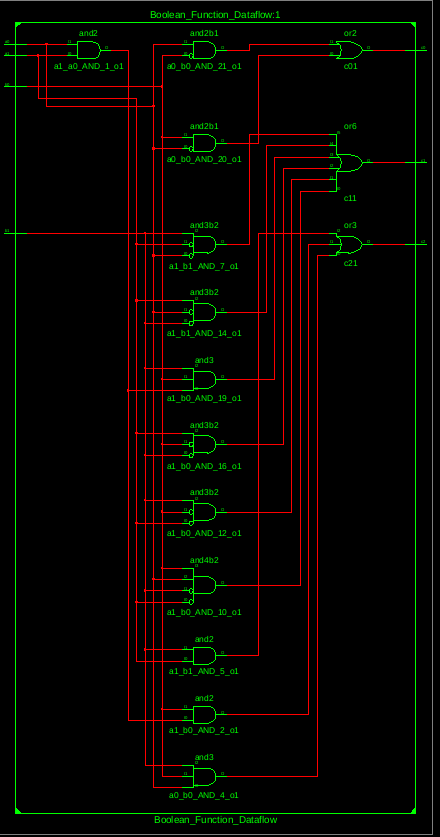
\includegraphics[width=0.7\textwidth]{img/rtl_df_2.png}
    \caption{RTL Schematic of the Components of the Boolean Function Data Flow}
    \label{fig:rtl-schematic-components-dataflow}

\end{figure}

\newpage

\subsubsection*{Simulation Results}

The simulation results of the testbench for the dataflow model is shown in Figure \ref{fig:simulation-results-dataflow}.

\begin{figure}[H]
    \centering
    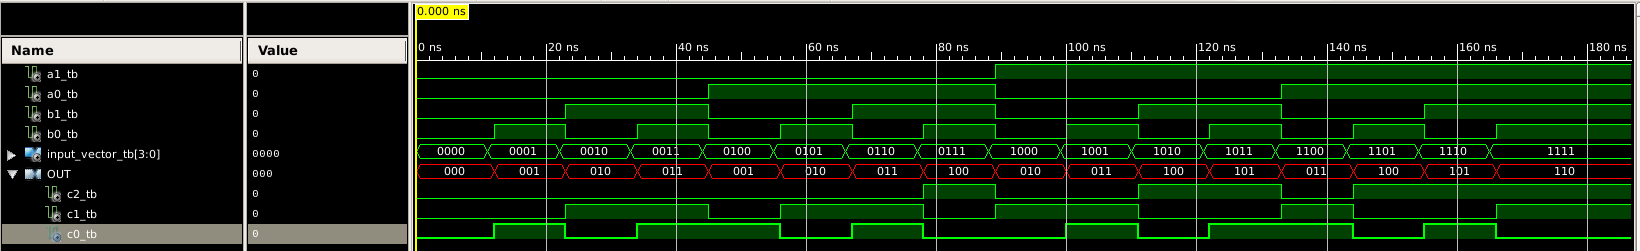
\includegraphics[width=1\textwidth]{img/dataflow_sim.png}
    \caption{Simulation Results of the Testbench for the Boolean Function Data Flow}
    \label{fig:simulation-results-dataflow}

\end{figure}

It can be seen that from inputs at the bottom of the waveform, the outputs \(c_2\), \(c_1\), and \(c_0\) are as expected from the truth table in Table \ref{tab:truth-given}.





\end{document}
